\chapter{Theoretical Background} % <<< --------------------------------------- %
\label{ch:app:theoretical_background}
% ---------------------------------------------------------------------------- %

\section{Internal Behavior of a CIC Filter} % <<< ---------------------------- %
\label{sec:app:cic_simu}
% ---------------------------------------------------------------------------- %

This  section presents  an example  for  a very  simple CIC  filter to  better
understand  its  internal  workings. For  verification,  the  filter  is  also
implemented in a Simulink model and simulated.

In the interest of simplicity, we choose  a filter with a decimation rate $R =
2$, a differential delay $M=1$ and $N=1$ stages. The corresponding topology is
shown in Figure~\ref{fig:cic_simu:topo}; Figure~\ref{fig:cic_simu:freqz} shows
the magnitude frequency  response of the filter. As can be  clearly seen, this
filter would be of very limited  use in practice. However, for the purposes of
this example, we  will feed a DC  signal (a constant) into the  filter, so the
only thing  of importance is  the filter's DC  gain (which is  \SI{6}{\dB}, or
\num{2}).

Lastly,  we  will   restrict  numerical  accuracy  to  three   bits  in  two's
complement;  the  entire  range  of  representable  values  can  be  found  in
Figure~\ref{fig:cic_simu:twos_complement_circle}. This  will limit  the number
of steps  which need  to be calculated  to gain the  desired insight  into the
filter's mathematical mechanics.

\begin{figure}
    \centering
    % https://tex.stackexchange.com/a/183092/131649
\tikzsetnextfilename{cicTopology}
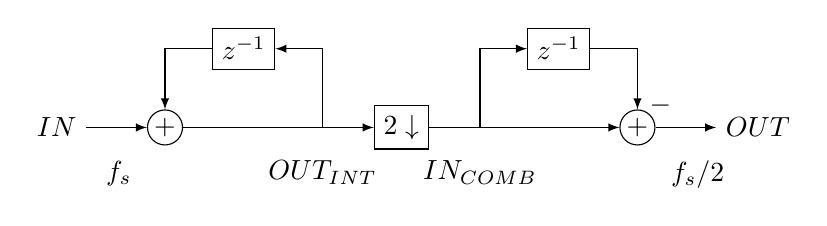
\begin{tikzpicture}
    \coordinate (in)  at (0,0);
    \coordinate (out) at (8,0);

    % branching coordinates
    \coordinate (b1) at (3,0);
    \coordinate (b2) at (5,0);

    % Delay elements
    \node[draw] (d1) at  (2,1) {$z^{-1}$};
    \node[draw] (d2) at  (6,1) {$z^{-1}$};

    % Downsampler
    \node[draw] (r1) at (4,0) {$2\downarrow$};

    % Adders
    \node[draw,circle, inner sep=0.3mm] (a1) at  (1,0) {$+$};
    \node[draw,circle, inner sep=0.3mm] (a2) at  (7,0) {$+$};

    % subtractors
    \node[above right=0.2ex] (s1) at (a2) {$-$};

    % Lines
    \draw[-latex] (in) -- (a1);
    \draw[-latex] (a1) -- (r1);
    \draw[-latex] (r1) -- (a2);
    \draw[-latex] (a2) -- (out);
    \draw[-latex] (b1) |- (d1);
    \draw[-latex] (b2) |- (d2);
    \draw[-latex] (d1) -| (a1);
    \draw[-latex] (d2) -| (a2);

    % Annotations
    \node[below left =2ex] at (a1) {$f_s$};
    \node[below right=2ex] at (a2) {$f_s/2$};
    \node[anchor=east] at (in) {$IN$};
    \node[anchor=west] at (out) {$OUT$};
    \node[anchor=north,below=2ex] at (b1) {$OUT_{INT}$};
    \node[anchor=north,below=2ex] at (b2) {$IN_{COMB}$};
\end{tikzpicture}

    \caption[Topology of Example Filter]{Topology of the CIC filter for this example}
    \label{fig:cic_simu:topo}
\end{figure}

\begin{figure}
    \centering
    \newcommand*\freqzFileInt{images/cicSimu/cic1.csv}
\pgfplotstableread[col sep=comma]{\freqzFileInt}\freqzTableInt
\begin{tikzpicture}[
        spy using outlines={magnification=4, connect spies}
    ]
     \pgfplotsset{every axis/.style={
            height=60mm,
            width=\textwidth,
            grid=none,
            y filter/.code={\pgfmathparse{20*log10(\pgfmathresult))}},
            x filter/.code={\pgfmathparse{\pgfmathresult / 3.141592654}},
            xticklabel style={font=\footnotesize},
            x unit=\times\,\pi\,\si{\radian}/\si{\sample},
            y unit=\si{dB},
            xlabel=Normalized Frequency,
            ylabel=Magnitude,
        },
        every axis legend/.append style={
            at={(1,-0.25)},  % if attached to bottom plot
            anchor=north east,
            cells={anchor=east},
        },
    }
    \begin{axis}[
            title=Integrator Frequency Responses,
            at = {(0,0)},
            xmin=0,
            xmax=1,
            xtick={0,0.5,1},
            ytick={6,0,-20,-40},
            xticklabels={0,$f_s/4$,$f_s/2$},
        ]
        \addplot[thick,q1,-] table[x=w, y=abs(H)] \freqzTableInt;
    \end{axis}
\end{tikzpicture}

    \caption[Frequency Respose of Example CIC Filter]{%
        Frequency response of a CIC  filter with $N=1$, $M=1$, $R=2$. Note the
        DC gain of \num{2}.%
    }
    \label{fig:cic_simu:freqz}
\end{figure}

The  state  of  the  filter  can  be  calculated  by  the  formulae  given  in
Equations~\ref{eq:cic_simu:INT} and \ref{eq:cic_simu:OUT}:
\begin{align}
    N             & = 1 \quad M = 1 \quad R=2\nonumber\\     
    OUT_{INT}[n]  & = IN_{COMB}[n] = IN[n]        + OUT[n-1] 
    \label{eq:cic_simu:INT} \\
    OUT_{COMB}[n] & = IN_{COMB}[n] - IN_{COMB}[n-R\cdot M] 
    \nonumber\\
                  & = OUT_{INT}[n] - OUT_{INT}[n-2] 
    \label{eq:cic_simu:OUT}
\end{align}

The  input  of the  filter  shall  be a  constant  of  $1$, starting  at  time
zero. Once this  input is  applied to  the system,  the integrator  stage will
begin  to  accumulate  the  constant. Given  an  unlimited  number  of  digits
(bits),  the integrator  would in  theory reach  infinity if  it kept  running
forever. In practice, however, it wraps around once it has reached its maximum
representable value  (\code{011}~$ =  3$) and begins  counting from  its lower
numerical limit  (\code{100}~$=-4$) again. This cycle keeps  repeating as long
as the filter is running.

The  ingenuinty of  the  CIC filter  lies  in exploiting  the  fact that  this
wraparound is irrelevant to the  comb stage. Whether the comb stage calculates
the difference between  an integrator's value whose precision  is unbounded or
whether it calculates the difference between two values which have potentially
been  wrapped  is  without  consequence.

As a  demonstration of this effect,  we shall examine the  computation step of
cycle $n = 4$  from Table~\ref{tab:cic_simu:cic_filter_states} (which contains
the  entire filter's  state for  15 steps). At  this point,  the state  of the
filter's output is  as follows (represented in three-bit  two's complement and
decimal):
\begin{align}
    OUT_{COMB}[4]_\mathrm{b} &= OUT_{INT}[4] - OUT_{INT}[2]     \nonumber\\
                             &= 101_\mathrm{b} - 011_\mathrm{b} \nonumber\\
                             &= 010_\mathrm{b}
    \label{eq:cic_simu:stage4:binary} \\
    OUT_{COMB}[4]_\mathrm{d} &= -3_\mathrm{d} - 3_\mathrm{d}    \nonumber\\
                             &= -6_\mathrm{d}
    \label{eq:cic_simu:stage4:decimal:bounded}
\end{align}
Obviously,   the  decimal   and   binary  results   do   not  match. This   is
where   the  wraparound   comes   into   play,  for   which   we  shall   look
at  Figure~\ref{fig:cic_simu:twos_complement_circle}. The  figure  presents  a
circular  arrangement  for   all  numbers  in  two's   complement  with  three
digits  precision.   In  that  arrangement,  addition  of  a  positive  number
corresponds to  moving clockwise  through the circle,  while subtraction  of a
positive number means moving  counterclockwise. Doing this for the calculation
of  Equation~\ref{eq:cic_simu:stage4:decimal:bounded},  we  find  that  moving
by  three  in  the  counterclockwise   direction  lands  us  at  $2$,  exactly
as   Equation~\ref{eq:cic_simu:stage4:binary}  demands. The   computation  has
\emph{wrapped around} its boundary ($-4$).

What     is     left    to     verify     is     that    the     result     of
Equation~\ref{eq:cic_simu:stage4:binary} is indeed the correct result, i.e. if
an  unbounded integrator  and comb  would have  yielded the  same outcome. And
indeed, they would have:
\begin{equation}
    \label{eq:cic_simu:stage4:decimal:unbounded}
    OUT_{COMB}[6] = 7 - 5 = 2
\end{equation}

\begin{figure}
    \centering
    \tikzsetnextfilename{twosComplementCircle}
\begin{tikzpicture}
    \node (b1) at   (0:2.5) {\texttt{010}};
    \node (b2) at  (45:2.5) {\texttt{001}};
    \node (b3) at  (90:2.5) {\texttt{000}};
    \node (b4) at (135:2.5) {\texttt{111}};
    \node (b5) at (180:2.5) {\texttt{110}};
    \node (b6) at (225:2.5) {\texttt{101}};
    \node (b7) at (270:2.5) {\texttt{100}};
    \node (b8) at (315:2.5) {\texttt{011}};

    \node (d1) at   (0:3.5) {\footnotesize$2$};
    \node (d2) at  (45:3.5) {\footnotesize$1$};
    \node (d3) at  (90:3.5) {\footnotesize$0$};
    \node (d4) at (135:3.5) {\footnotesize$-1$};
    \node (d5) at (180:3.5) {\footnotesize$-2$};
    \node (d6) at (225:3.5) {\footnotesize$-3$};
    \node (d7) at (270:3.5) {\footnotesize$-4$};
    \node (d8) at (315:3.5) {\footnotesize$3$};

    \draw[thick,q5,-latex]
        (b6)
        edge[out=315,in=180]
        node[midway,anchor=north east] {\texttt{-1}}
        (b7);
    \draw[thick,q5,-latex]
        (b7)
        edge[out=  0,in=225]
        node[midway,anchor=north] {\texttt{-1}}
        (b8);
    \draw[thick,q5,-latex]
        (b8)
        edge[out= 45,in=270]
        node[midway,anchor=north west] {\texttt{-1}}
        (b1);

    \draw[thick,q5,-latex] (0:1.5) arc[start angle= 0, end angle= 240, radius=1.5cm];
    \draw[thick,q1,-latex] (60:1.0) arc[start angle=60, end angle=-180, radius=1.0cm];

    \node at (120:1.25) {\color{q5}$-$};
    \node at (-60:0.75) {\color{q1}$+$};
\end{tikzpicture}

    \caption[Two's Complement Circle]{%
        Subtracting  $3$  from $-3$  in  two's  complement with  three  digits
        precicion,  represented on  a  circle. Addition of  a positive  number
        corresponds  to moving  clockwise,  subtraction of  a positive  number
        corresponds to moving counterclockwise.%
    }
    \label{fig:cic_simu:twos_complement_circle}
\end{figure}

\begin{table}
    \centering
    \caption[CIC Filter Example: States for 16 Cycles]{%
        Binary and  decimal values  for the  different filter  elements during
        various  stages  of the  filtering  process. As  expected due  to  the
        filter's DC  gain of  \num{2}, its output  is indeed  \num{2}. The two
        right  columns contain  the calculations  as they  would occur  if the
        filter's components had  unbounded precision. It can be  seen that the
        wraparound effect  of the two's complement  representation does indeed
        not change the filter's output.%
    }
    \label{tab:cic_simu:cic_filter_states}
    \ttfamily
    \begin{tabular}{rrrr|rrr}
        \toprule
        \scshape Cycle                   &
        \scshape IN                      &
        \scshape OUT\textsubscript{INT}  &
        \scshape OUT                     &
        \scshape OUT\textsubscript{INT}  &
        \scshape OUT                     &
        \scshape OUT                     \\

        &
        &
        \scshape IN\textsubscript{COMB} &
        &
        (unbounded) &
        (bounded    &
        (unbounded  \\

        &
        &
        &
        &
        &
        integrator) &
        integrator) \\

        \midrule
        %     IN   OI/IC  OUT   UW
        -2 & 000 &  000 & 000 & $ 0$ &                                    & \\
        -1 & 000 &  000 & 000 & $ 0$ &                                    & \\
         0 & 001 &  001 & 001 & $ 1$ & $  1 -   0  =  1                 $ & $ 1 - 0 = 1 $\\
         1 & 001 &  010 &     & $ 2$ &                                    & \\
         2 & 001 &  011 & 010 & $ 3$ & $  3 -   1  =  2                 $ & $ 3 - 1 = 2 $\\
         3 & 001 &  100 &     & $ 4$ &                                    & \\
         4 & 001 &  101 & 010 & $ 5$ & $ -3 -   3  = -6 = 2_\mathrm{wr} $ & $ 5 - 3 = 2 $\\
         5 & 001 &  110 &     & $ 6$ &                                    & \\
         6 & 001 &  111 & 010 & $ 7$ & $ -1 - (-3) =  2                 $ & $ 7 - 5 = 2 $\\
         7 & 001 &  000 &     & $ 8$ &                                    & \\
         8 & 001 &  001 & 010 & $ 9$ & $  1 - (-1) =  2                 $ & $ 9 - 7 = 2 $\\
         9 & 001 &  010 &     & $10$ &                                    & \\
        10 & 001 &  011 & 010 & $11$ & $  3 -   1  =  2                 $ & $ 11 - 9 = 2 $\\
        11 & 001 &  100 &     & $12$ &                                    & \\
        12 & 001 &  101 & 010 & $13$ & $ -3 -   3  = -6 = 2_\mathrm{wr} $ & $ 13 - 11 = 2 $\\
        13 & 001 &  110 &     & $14$ &                                    & \\
        14 & 001 &  111 & 010 & $15$ & $ -1 - (-3) =  2                 $ & $ 15 - 13 = 2 $\\
        \bottomrule
    \end{tabular}
\end{table}

As  a   last  step   to  confirm   our  results,  the   CIC  filter   of  this
exercise  is   simulated  with   Simulink. Its  block   design  is   given  in
Figure~\ref{fig:cic_simu:simulink_model}. All   blocks   are  set   to   two's
complement with three digits of precision (no fractional bits).

The          simulation         results          are         given          in
Figure~\ref{fig:cic_simu:simulink_results}. As can be  seen, the filter states
are  identical  to   our  manually  calculated  example. The   effect  of  the
integrator's output  wrapping around the  numerical boundaries is  also nicely
visible.

TODO: Give file path

\begin{figure}
    \centering
    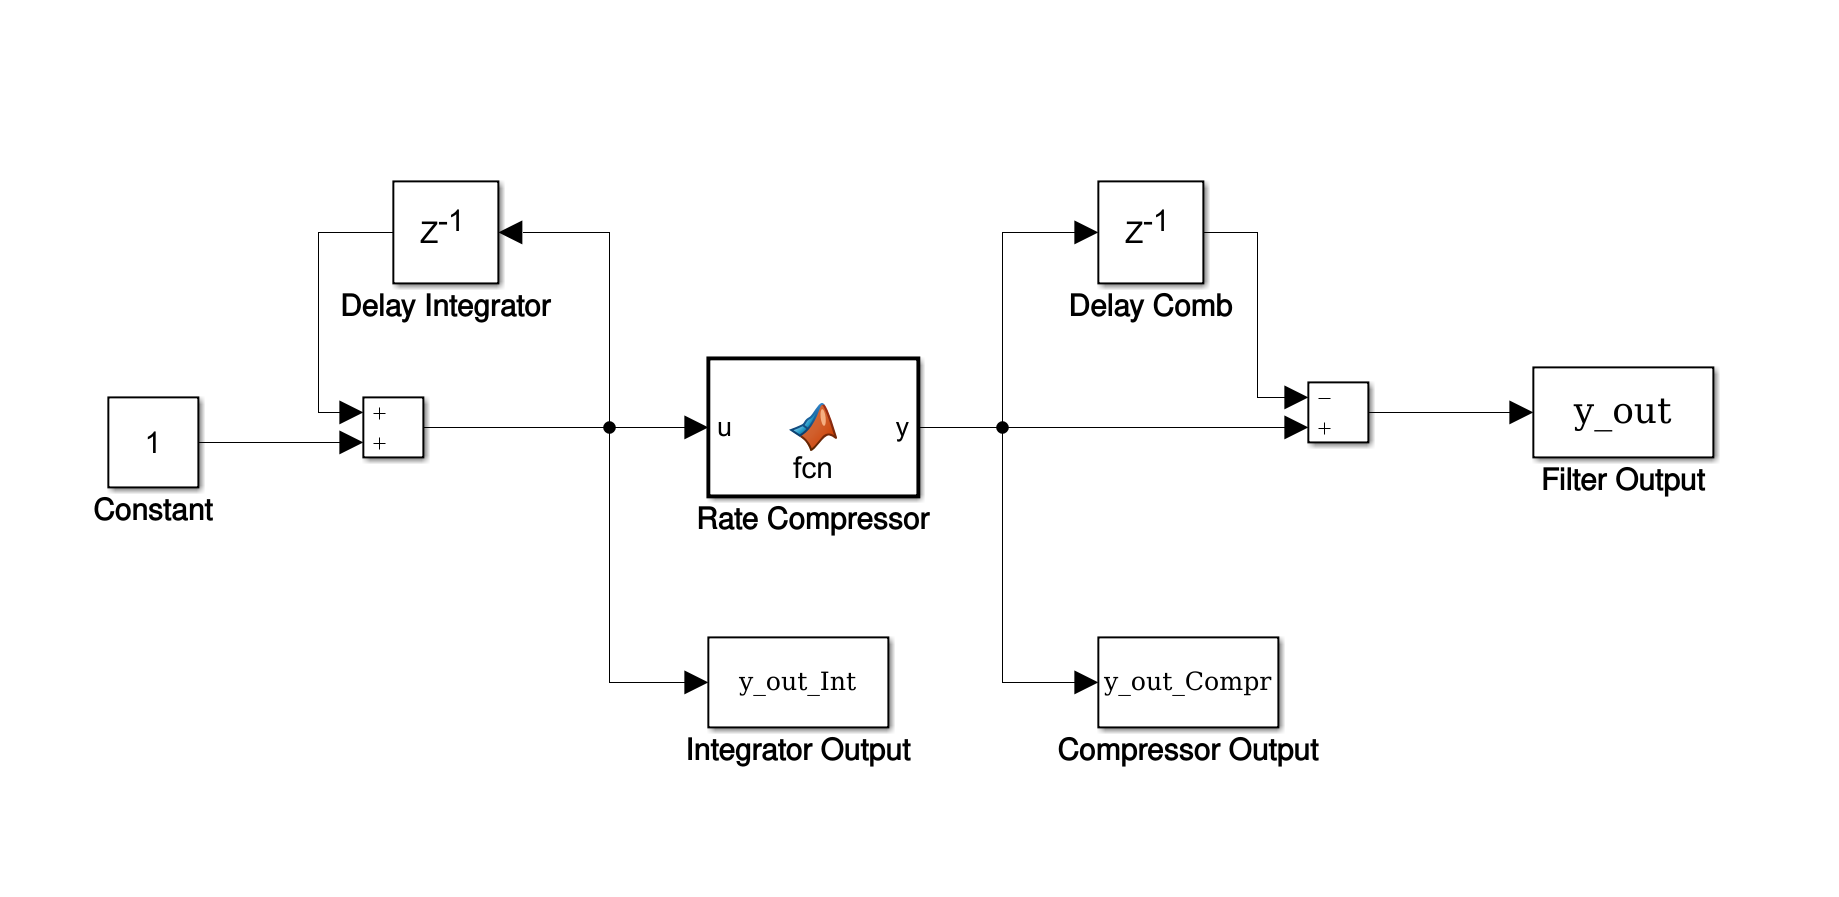
\includegraphics[width=\textwidth]{images/cicSimu/simulink.png}
    \caption[Simulink Filter Model]{%
        Simulink model  for the filter  in Figure~\ref{fig:cic_simu:topo}. The
        Rate   Compressor is  a  simple Matlab  function  which returns  every
        second value of its input vector.%
    }
    \label{fig:cic_simu:simulink_model}
\end{figure}

\begin{figure}
    \centering
    \newcommand*\freqzFileIntA{images/cicSimu/simulinkYout.csv}
\newcommand*\freqzFileIntB{images/cicSimu/simulinkYoutCompr.csv}
\newcommand*\freqzFileIntC{images/cicSimu/simulinkYoutInt.csv}
\pgfplotstableread[col sep=comma]{\freqzFileIntA}\freqzTableIntA
\pgfplotstableread[col sep=comma]{\freqzFileIntB}\freqzTableIntB
\pgfplotstableread[col sep=comma]{\freqzFileIntC}\freqzTableIntC
\begin{tikzpicture}
    \pgfplotsset{every axis/.style={
            height=50mm,
            width=\textwidth,
            grid=none,
            xmin=-1,
            xmax=15,
            xtick={0,2,4,6,8,10,12,14},
            ytick={-4,-2,0,2,4},
            ylabel=$OUT$,
            xlabel=$n$,
        },
    }
    \begin{axis}[
            title=Filter Output,
            at = {(0,0)},
            ytick={0,1,2},
            ymin=0,
        ]
        \addplot[ycomb,mark=*,dv+5,-] table[x=t,y=y] \freqzTableIntA;
    \end{axis}

    \begin{axis}[
            title=Compressor Output (Comb Input),
            at = {(0,-55mm)},
            ymin=-4,
            ymax=4,
        ]
        \addplot[ycomb,mark=*,dv+5,-] table[x=t,y=y] \freqzTableIntB;
        \draw[gray] (rel axis cs:0,0.5) -- (rel axis cs:1,0.5);
    \end{axis}

    \begin{axis}[
            title=Integrator Output,
            at = {(0,-110mm)},
            ymin=-5,
            ymax=4,
        ]
        \addplot[ycomb,mark=*,dv+5,-] table[x=t,y=y] \freqzTableIntC;
        \draw[gray] (-1,0) -- (15,0);
    \end{axis}
\end{tikzpicture}

    \caption[Simulink Simulation Results]{%
        Simulation    results    from    Simulink   for    the    filter    in
        Figure~\ref{fig:cic_simu:simulink_model}.%
    }
    \label{fig:cic_simu:simulink_results}
\end{figure}

Lastly,  it is  shown what  happens  when the  expected output  of the  filter
exceeds  the numerical  range  available. This is  accomplished  by feeding  a
constant of \num{2} into the filter; the expected output is therefore \num{4}.

Because \num{4}  is not  within the  range of  a three-digit  two's complement
number  system, the  filter wraps  around  and produces  an incorrect  output,
\num{-4}.   The  first  few  calculation  steps  for  this  are  presented  in
Table~\ref{tab:cic_simu:cic_filter_states:out_of_bounds};  running  the  above
simulation with the modified input also comfirms this result.

\begin{table}
    \centering
    \caption[CIC Filter Example: Output Out of Range]{%
        The  same CIC  filter  as  before stimulated  with  an  input of  2. A
        comparison between the right two columns  shows that the output of the
        bounded filter and its unbounded  counterpart no longer match starting
        with the output at $n=2$; the filter produces a false output.%
    }
    \label{tab:cic_simu:cic_filter_states:out_of_bounds}
    \ttfamily
    \begin{tabular}{rrrr|rrr}
        \toprule
        \scshape Cycle                   &
        \scshape IN                      &
        \scshape OUT\textsubscript{INT}  &
        \scshape OUT                     &
        \scshape OUT\textsubscript{INT}  &
        \scshape OUT                     &
        \scshape OUT                     \\

        &
        &
        \scshape IN\textsubscript{COMB} &
        &
        (unbounded) &
        (bounded    &
        (unbounded  \\

        &
        &
        &
        &
        &
        integrator) &
        integrator) \\

        \midrule
        %     IN   OI/IC  OUT   UW
        -2 & 000 &  000 & 000 & $ 0$ &                        & \\
        -1 & 000 &  000 & 000 & $ 0$ &                        & \\
         0 & 010 &  010 & 010 & $ 2$ & $  2 -   0  =  2     $ & $ 2 - 0 = 2 $\\
         1 & 010 &  100 &     & $ 4$ &                        & \\
         2 & 010 &  110 & 100 & $ 6$ & $ -2 -   2  = -4     $ & $ 6 - 2 = 4 $\\
         3 & 010 &  000 &     & $ 8$ &                        & \\
         4 & 010 &  010 & 100 & $10$ & $  2 - (-2) = -4     $ & $10 - 6 = 4 $\\
        \bottomrule
    \end{tabular}
\end{table}
%>>>

\section{CIC Filter Tables} % <<< -------------------------------------------- %
\label{sec:app:cic_filter_tables}
% ---------------------------------------------------------------------------- %

\begin{table}
    \centering
    \caption[CIC Filter Passband Attenuations]{%
        Passband    attenuation    for    CIC   filters    as    a    function
        of   the   bandwidth-differential    delay   product. Taken   directly
        from~\cite{1163535}.%
    }
    \label{tab:cic:pb_attenuation}
    \begin{tabular}{rrrrrrrr}
        \toprule
            \parbox[t]{40mm}{
                Relative \\
                Bandwidth-Differential\\
                Delay Product ($Mf_c$)} &
            \multicolumn{7}{c}{\parbox[t]{60mm}{
                Passband attenuation at $f_c$ in \si{\dB} \\
                as a Function of \\
                Number of Stages ($N$)}}                                  \\
        \midrule
            & 1 & 2 & 3 & 4 & 5 & 6 \\
        \midrule
            $1/128$ & $0.00$ & $0.00$ & $0.00$ & $0.00$ & $0.00$ & $0.01$ \\
            $1/64 $ & $0.00$ & $0.01$ & $0.01$ & $0.01$ & $0.02$ & $0.02$ \\
            $1/32 $ & $0.01$ & $0.03$ & $0.04$ & $0.06$ & $0.07$ & $0.08$ \\
            $1/16 $ & $0.06$ & $0.11$ & $0.17$ & $0.22$ & $0.28$ & $0.34$ \\
            $1/8  $ & $0.22$ & $0.45$ & $0.67$ & $0.90$ & $1.12$ & $1.35$ \\
            $1/4  $ & $0.91$ & $1.82$ & $2.74$ & $3.65$ & $4.56$ & $5.47$ \\
        \bottomrule
    \end{tabular}
\end{table}

\begin{table}
    \centering
    \caption[CIC Filter Passband Aliasing Attenuation]{%
        Passband  aliasing   attenuation  for   CIC  filters  as   a  function
        of   the  bandwidth   and  the   differential  delay. Taken   directly
        from~\cite{1163535}.%
    }
    \label{tab:cic:pb_aliasing}
    \begin{tabular}{rrrrrrrrr}
        \toprule
            \parbox[t]{20mm}{
                Differential\\
                Delay\\
                ($M$)%
            } &
            \parbox[t]{20mm}{
                Relative \\
                Bandwidth\\
                ($f_c$)} &
            \multicolumn{7}{c}{\parbox[t]{70mm}{
                Aliasing/Imaging Attenuation at $f_\mathrm{s,low}$ in \si{\dB}\\
                as a Function of Number of Stages ($N$)}}\\
        \midrule
            & & 1 & 2 & 3 & 4 & 5 & 6 \\
        \midrule
            1 & $1/128$ & $42.1$ & $84.2$ & $126.2$ & $168.3$ & $210.4$ & $252.5$ \\
            1 & $1/64 $ & $36.0$ & $72.0$ & $108.0$ & $144.0$ & $180.0$ & $215.9$ \\
            1 & $1/32 $ & $29.8$ & $59.7$ & $ 89.5$ & $119.4$ & $149.2$ & $179.0$ \\
            1 & $1/16 $ & $23.6$ & $47.2$ & $ 70.7$ & $ 94.3$ & $117.9$ & $141.5$ \\
            1 & $1/8  $ & $17.1$ & $34.3$ & $ 51.4$ & $ 68.5$ & $ 85.6$ & $102.8$ \\
            1 & $1/4  $ & $10.5$ & $20.9$ & $ 31.4$ & $ 41.8$ & $ 52.3$ & $ 62.7$ \\
        \midrule
            2 & $1/256$ & $48.1$ & $96.3$ & $144.4$ & $192.5$ & $240.7$ & $288.8$ \\
            2 & $1/128$ & $42.1$ & $84.2$ & $126.2$ & $168.3$ & $210.4$ & $252.5$ \\
            2 & $1/64 $ & $36.0$ & $72.0$ & $108.0$ & $144.0$ & $180.0$ & $216.0$ \\
            2 & $1/32 $ & $29.9$ & $59.8$ & $ 89.6$ & $119.5$ & $149.4$ & $179.3$ \\
            2 & $1/16 $ & $23.7$ & $47.5$ & $ 71.2$ & $ 95.0$ & $118.7$ & $179.3$ \\
            2 & $1/8  $ & $17.8$ & $35.6$ & $ 53.4$ & $ 71.3$ & $ 89.1$ & $106.9$ \\
        \bottomrule
    \end{tabular}
\end{table}
%>>>
%>>>

%^^A vim: foldenable foldcolumn=4 foldmethod=marker foldmarker=<<<,>>>
